\chapter{Modèle vectoriel}
\section{Introduction}
Le modèle vectoriel (Vector Space Model) est l'une de modèle le plus utilisé en recherche d'information, que ce soit textuel \Citep{sarch-engine-vsm} ou multimédia \citep{vsm-images}. Ce modèle est apparu lorsque la pondération binaire est limitant, et que l'appariement partielle n'est pas possible, en introduisant la pondération non binaire et un appariement partielle \citep{modern-ir}.

Ce modèle a comme principe la modélisation de la requête et des documents sous forme d'un vecteur, pondérer les termes dans ce vecteur avec des méthodes de pondération comme le \emph{TF-IDF}, et calcule ensuite la distance euclidienne entre les vecteurs documents et la vecteur requête pour déterminer la pertinence \citep{ir-on-web}. Un score de similarité est alors calculé pour pouvoir classer les documents jugés pertinent par le système. La représentation du document et la requête est illustré dans la Figure~\ref{fig:vector-model}. Ce modèle est introduit dans la Section~\ref{sec:vsm-model}.

\begin{definition}[Modèle Véctoriel]
    On note $w_{ij}$ le poids positif et non binaire, du terme $i$ dans le document $j$ qui est associé avec un pair $(k_{i}, d_{j})$ et $w_{iq}$ le poids du terme $i$ dans la requête $q$. La requête est définie par le vecteur: $ \vec{q} = (w_{1q}, w_{2q}, \dots, w_{tq}) $ où $t$ le nombre total des termes d'indexation dans le système. Un document $d_{j}$ est présenté par le vecteur: $ \vec{d_{j}} = (w_{1j}, w_{2j}, \dots, w_{tj}) $.

    La calcul de similarité entre ces deux vecteurs se traduit par la formule:
    \[
        Sim(\vec{d}, \vec{q}) = \frac{\vec{d_{j}} \cdot \vec{q}}{ |\vec{d_{j}}| \times |\vec{q}| } \\
        = \frac{\sum_{i=1}^{t} w_{i,j} \times w_{i,q}}{\sqrt{\sum_{i=1}^{t} (w_{i,j})^2} \times \sqrt{\sum_{i=1}^{t} (w_{i,q})^2}}
    \]

    Avec $ |\vec{d_{j}}| $ et $ |\vec{q}| $ norme du vecteur document et de la vecteur requête.
\end{definition}

\section{Problème de classification}
Ce problème est illustré et analyser dans \citep{modern-ir}. L'étude de Salton définit la problème de RI comme un problème de classification. Notons une collection de document \emph{C} et que la requête de l'utilisateur est une vague représentation de l'ensemble des documents \emph{A}. Le problème est donc de déterminer quelle documents appartient a l'ensemble \emph{A}, qui est un problème de classification.

Dans un problème de classification, il y a deux problème: la première consiste a déterminer les fonctionnalités qui décrit le mieux les objets dans la collection \emph{A}; et la seconde consiste a déterminer les fonctionnalités qui distingue les objets dans collection \emph{A} pour les autres objets provenant de la collection \emph{C}. La première fonctionnalité produit la quantification \emph{intra-clustering} tandis que la seconde fonctionnalité produit la quantification \emph{inter-clustering}.

Dans le modèle vectoriel, la similarité \emph{intra-clustering} est quantifié par la mesure de la fréquence du terme $k_{i}$ dans le document $d_{j}$. Cette facteur est souvent appelé facteur \emph{tf} ou \emph{term frequency}, qui décrit la caractérisation \emph{intra-document}. D'autre part, la similarité \emph{inter-clustering} est quantifié par la mesure de l'inverse du fréquence du terme $k_{i}$ parmi les documents dans la collection. Cette facteur est souvent appelé facteur \emph{idf} ou \emph{inverse document frequency}

Pour avoir un meilleur classification des documents, il faut balancer ces deux mesures.

\section{Méthodes de pondération des termes}
Cette facteur est permet de calculer la fréquence d'un terme dans un document, voir Section~\ref{sec:mesure-similarite}.

\begin{definition}
    Cette définition est tiré de \citetitle{modern-ir} \Citep{modern-ir}. Notons \emph{N} le nombre total des documents dans le système et $n_{i}$ le nombre de documents contenant le terme $k_{i}$. Notons $freq_{i,j}$ la fréquence du terme $k_{i}$ dans le document $d_{j}$ (le nombre de dois où le terme $k_{i}$ est mentionné dans le texte du document $d_{j}$). Alors la fréquence normalisé $f_{i,j}$ du terme $k_{i}$ dans le document $d_{j}$ est donné par
    \[
        f_{i,j} = \frac{freq_{i,j}}{\max_{l} freq_{i,j}}
    \]

    où le maximum est calculé a travers les termes qui sont mentionné dans le texte du document $d_{j}$. Si le terme $k_{i}$ n'appartient pas au document $d_{j}$ alors $f_{i,j} = 0$. D'autre part, notons $idf_{i}$ l'\emph{inverse document frequency} pour le terme $k_{i}$, qui est donné par
    \[
        idf_{i} = \log{\frac{N}{n_{i}}}
    \]

    La pondération de terme le plus connu et plus utilisé est donné par
    \[
        w_{i,j} = f_{i,j} \times \log{\frac{N}{n_{i}}}
    \]
    ou par la variation de ce formule. Ce pondération de termes est aussi appelé facteur \emph{tf-idf}
\end{definition}

Certains variations de ce méthode de pondération est introduit en 1988, mais la formule précédente est efficace pour la plupart des collection. Pour la requête, Salton et Buckley \Citep{modern-ir} a suggéré la pondération suivante
\[
    w_{i,q} = \left(0.5 + \frac{0.5 freq_{i,q}}{\max_{l} freq_{i,j}}\right) \times \log{\frac{N}{n_{i}}}
\]

\section{Variant du TF-IDF}
Les variants de ces méthodes sont illustré dans la Tableau~\ref{tab:variant-tf} qui est celle de la \emph{tf}, la Tableau~\ref{tab:variant-idf} qui est celle de l'\emph{idf} et la Tableau~\ref{tab:variant-tf-idf} qui est celle de \emph{tf-idf}.

\begin{table}[htbp]
    \centering
    \renewcommand{\arraystretch}{1.5} % Specify the line height here
    \begin{tabularx}{\textwidth}{|X|X|}
        \hline
        \textbf{Weighting sheme} & \textbf{TF weight} \\
        \hline
        Binary & 0, 1 \\
        \hline
        Raw count & $f_{t,d}$ \\
        \hline
        Term frequency & $f_{t,d} \left/ \sum_{t' \in d} f_{t',d} \right.$ \\
        \hline
        Log normalization & $\log{(1 + f_{t,d})}$ \\
        \hline
        Double normalization 0.5 & $ 0.5 + 0.5 \cdot \frac{f_{t,d}}{\max_{t' \in d} } f_{t',d}$ \\
        \hline
        Double normalization K & $ K + K \cdot \frac{f_{t,d}}{\max_{t' \in d} } f_{t',d}$ \\
        \hline
    \end{tabularx}
    \caption{Variant du TF \citep{sarch-engine-vsm}}\label{tab:variant-tf}
\end{table}

\begin{table}[htbp]
    \centering
    \renewcommand{\arraystretch}{1.5} % Specify the line height here
    \begin{tabularx}{\textwidth}{|X|X|}
        \hline
        \textbf{Weighting sheme} & \textbf{IDF ($ n_{i} = \left| \{d \in D: t \in d\} \right| $)} \\
        \hline
        Unary & 1 \\
        \hline
        Inverse document frequency & $ \log{\frac{N}{n_{t}}} = -log{\frac{n_{t}}{N}} $ \\
        \hline
        Inverse document frequency smooth & $ \log{\left( \frac{N}{1 + n_{t}} \right)} + 1 $ \\
        \hline
        Inverse document frequency max & $ \log{\left( \frac{\max_{\{ t' \in d \}} n_{t'}}{1 + n_{t}} \right)} $ \\
        \hline
        Log normalization-idf & $ (1 + \log{f_{t,d}}) \cdot \log{\frac{N}{n_{t}}} $ \\
        \hline
    \end{tabularx}
    \caption{Variant de l'IDF \citep{sarch-engine-vsm}}\label{tab:variant-idf}
\end{table}

\begin{table}[htbp]
    \centering
    \renewcommand{\arraystretch}{1.5} % Specify the line height here
    \begin{tabularx}{\textwidth}{|X|X|}
        \hline
        \textbf{Weighting sheme} & \textbf{TF-IDF} \\
        \hline
        Count-idf & $ f_{t,d} \cdot \log{\frac{N}{n_{t}}} $ \\
        \hline
        Double normalization-idf & $ \left( 0.5 + 0.5 \cdot \frac{f_{t,q}}{\max_{t} f_{t,q}} \right) \log{\frac{N}{n_{t}}} $ \\
        \hline
        Log normalization-idf & $ (1 + \log{f_{t,d}}) \cdot \log{\frac{N}{n_{t}}} $ \\
        \hline
    \end{tabularx}
    \caption{Variant du TF-IDF \citep{sarch-engine-vsm}}\label{tab:variant-tf-idf}
\end{table}

\section{Document inversé}
Un \emph{document inversé} ou \emph{fichier inversé} est un structure de données au cœur des moteurs de recherche gigantesque, des réseaux sociaux et des architectures de stockage. Il permet de stocker des millions des documents \citep{techniques-compression-inverted-index}.

\begin{definition}[Fichier inversé]
    Considérons une collection des documents textuels, et que chacun est décrit comme un ensemble des termes. Pour chaque terme distinct $t$ qui apparaissant dans la collection, un séquence d'entier $S_{t}$ est crée et répertorie, dans l'ordre trié, tous les identifiants des documents (dorénavant, docIDs) où le terme apparaît. La séquence $S_{t}$ est appelé liste inversé ou \emph{posting list} pour le terme $t$ \citep{techniques-compression-inverted-index}.
\end{definition}

Le fichier inversé peut stocker des informations additionnel pour chaque terme, comme les positions du termes dans la document, le nombre d’occurrence du terme dans le document (fréquences).

Un exemple d'un fichier inversé est illustré dans la Figure~\ref{fig:inverted-indexes}.
\begin{figure}[htbp]
	\begin{center}
		\fbox{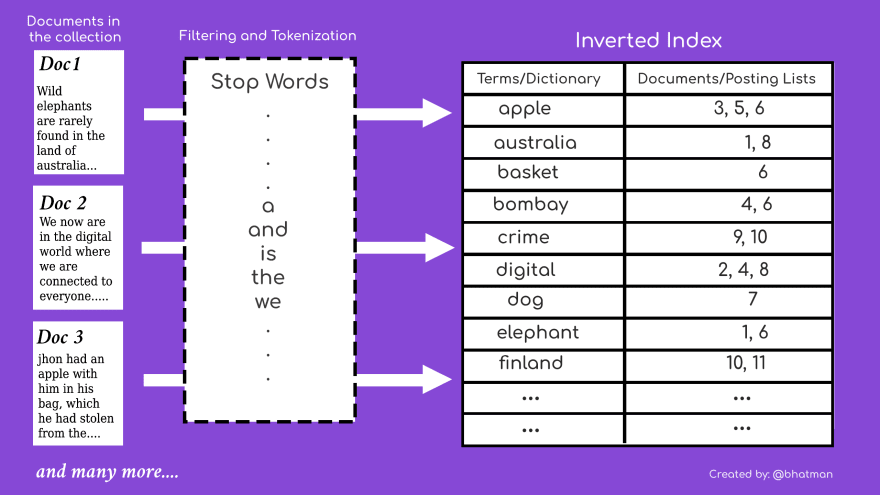
\includegraphics[width=15cm, angle=0]{Figures/VSM/inverted-indexes.png}}
	\end{center}
	\caption{Variant du TF-IDF \citep{inverted-indexes}}\label{fig:inverted-indexes}
\end{figure}

\section{Avantages}
Le modèle vectoriel ont les avantages suivantes \citep*{approche-semantique, soulier2014:def-evaluation-modele}:
\begin{itemize}
    \item \textbf{Facile a mettre en œuvre}: ce modèle est facile a implémenter en informatique, grâce a ces différentes formules ainsi que le fichier inversé.
    \item \textbf{Appariement partielle}: ce modèle propose la possibilité de faire une appariement approximatif avec un degré de pertinence. En d'autre terme, l'utilisateur reçoit des documents qui pourra satisfaire la moitié de la requête ou en quelque pourcentage.
    \item \textbf{Organisation des résultats}: comme l'appariement partielle est possible, les documents retournés sont alors organisé selon leur degré de pertinence décroissant afin de faciliter la selection des documents par l'utilisateur. L'utilisateur passe moins de temps donc a juger les résultats.
    \item \textbf{Définir une limite de pertinence}: ainsi ce modèle permet de définir une seuil pour calculer la pertinence afin que les documents ayant la pertinence inférieur a ce seuil ne sont pas retournés.
\end{itemize}

C'est grâce a ces avantages que ce modèle est populaire, et qu'il est le plus utilisé par les moteurs de recherche actuel.

\section{Inconvénients}
Par contre ce modèle a certaines lacunes \Citep{modern-ir, vsm}:
\begin{itemize}
    \item \textbf{Indépendance des termes d'indexation}: ce qui implique que la notion sémantique du document est perdu. Mais ce problème a été solutionné par la mise place de regroupement des termes qui ont la même sens, on l'appelle \emph{N-grammes}. Ou bien une autre approche est d'utiliser le modèle d’indexation sémantique latente (Latent Semantic Index).
    \item \textbf{Pas de théorie réelle}: il n'existe pas de base théorique réelle pour l'hypothèse d'un espace de termes.
    \item \textbf{Pondération des termes}: le poids associé aux vecteurs est totalement arbitraire, et que c'est un système indépendant.
\end{itemize}

\section{Conclusion}
Le modèle vectoriel est l'un de modèle le plus populaire dans la recherche d'information que ce soit textuel ou multimédia. Ce modèle est populaire grâce a son système de pondération non binaire (\emph{tf, idf, tf-idf}), la possibilité de faire une appariement partielle ainsi que le classement des résultats. Ce modèle propose différentes mesure de similarité pour l’appariement \emph{document-requête}, ainsi des variation pour le système de pondération. Le modèle vectoriel stock les documents dans le fichier inversé pour appliquer la recherche.